\begin{center}
    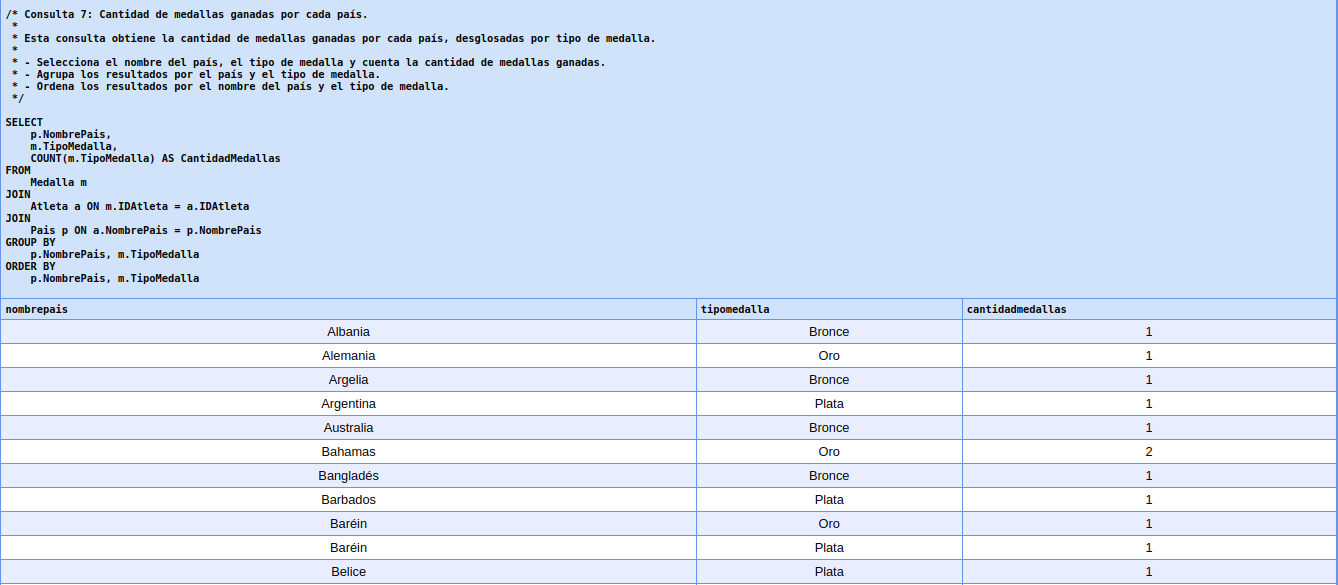
\includegraphics[width=16.5cm]{../resources/Chapters/Consultas/Imagenes/Consulta7.png} 
    
   Consulta 7: Cantidad de medallas ganadas por cada país.
\end{center}

\textbf{Propósito de la consulta}

La consulta tiene como objetivo obtener la cantidad de medallas ganadas por cada país, desglosadas por tipo de medalla (oro, plata o bronce). Esto proporciona una visión detallada del desempeño de cada nación en términos de premios obtenidos.

\textbf{Desglose de la consulta}

\begin{itemize}
   \item \textbf{Selección de columnas (\texttt{SELECT}):}
   \begin{itemize}
       \item \texttt{p.NombrePais}: Nombre del país al que pertenece el atleta ganador de la medalla.
       \item \texttt{m.TipoMedalla}: Tipo de medalla ganada (oro, plata o bronce).
       \item \texttt{COUNT(m.TipoMedalla) AS CantidadMedallas}: Cuenta la cantidad total de medallas ganadas por cada país, desglosadas según el tipo de medalla.
   \end{itemize}

   \item \textbf{Tablas involucradas (\texttt{FROM} y \texttt{JOIN}):}
   \begin{itemize}
       \item \texttt{Medalla (m)}: Contiene información sobre las medallas ganadas, incluyendo el tipo de medalla y el atleta que la ganó.
       \item \texttt{Atleta (a)}: Contiene información sobre los atletas, incluyendo su país de origen.
       \item \texttt{Pais (p)}: Contiene información sobre los países y sus nombres.
       \item \textbf{Uniones (\texttt{JOIN}):}
       \begin{itemize}
           \item Se realiza un \texttt{JOIN} entre \texttt{Medalla} y \texttt{Atleta} mediante la relación \texttt{m.IDAtleta = a.IDAtleta}, para asociar cada medalla con el atleta que la ganó.
           \item Se realiza otro \texttt{JOIN} entre \texttt{Atleta} y \texttt{Pais} mediante la relación \texttt{a.NombrePais = p.NombrePais}, para asociar cada atleta con su país de origen.
       \end{itemize}
   \end{itemize}

   \item \textbf{Agrupación de resultados (\texttt{GROUP BY}):}
   \begin{itemize}
       \item La agrupación se realiza por:
       \begin{itemize}
           \item \texttt{p.NombrePais}: Para obtener los resultados específicos de cada país.
           \item \texttt{m.TipoMedalla}: Para desglosar las medallas ganadas por tipo (oro, plata o bronce).
       \end{itemize}
       \item Esto permite contar las medallas de manera independiente para cada combinación de país y tipo de medalla.
   \end{itemize}

   \item \textbf{Ordenamiento de resultados (\texttt{ORDER BY}):}
   \begin{itemize}
       \item Los resultados se ordenan por:
       \begin{itemize}
           \item \texttt{p.NombrePais}: Los países se listan en orden alfabético.
           \item \texttt{m.TipoMedalla}: Dentro de cada país, los tipos de medalla se ordenan alfabéticamente (por ejemplo, bronce, oro, plata).
       \end{itemize}
   \end{itemize}
\end{itemize}

\textbf{Análisis detallado}

\begin{itemize}
   \item \textbf{Relación entre tablas:}
   \begin{itemize}
       \item La consulta utiliza tres tablas relacionadas:
       \begin{itemize}
           \item \texttt{Medalla}: Relaciona las medallas ganadas con los atletas que las obtuvieron.
           \item \texttt{Atleta}: Relaciona a los atletas con sus países de origen.
           \item \texttt{Pais}: Proporciona información sobre los países.
       \end{itemize}
       \item Las relaciones entre las tablas permiten obtener una asociación entre las medallas ganadas y los países correspondientes.
   \end{itemize}

   \item \textbf{Uso de la función agregada \texttt{COUNT}:}
   \begin{itemize}
       \item La función \texttt{COUNT(m.TipoMedalla)} cuenta la cantidad de medallas ganadas para cada combinación de país y tipo de medalla.
       \item Esto permite obtener un desglose detallado de las medallas (oro, plata y bronce) ganadas por cada país.
   \end{itemize}

   \item \textbf{Agrupación por columnas clave:}
   \begin{itemize}
       \item La agrupación por \texttt{p.NombrePais} y \texttt{m.TipoMedalla} asegura que las medallas se cuenten de manera específica para cada país y tipo de medalla.
   \end{itemize}

   \item \textbf{Ordenamiento por país y tipo de medalla:}
   \begin{itemize}
       \item Ordenar los resultados por \texttt{p.NombrePais} en orden alfabético facilita la lectura y comparación entre países.
       \item Ordenar por \texttt{m.TipoMedalla} dentro de cada país organiza los resultados por tipo de medalla (bronce, oro, plata).
   \end{itemize}
\end{itemize}

\textbf{Posibles escenarios y consideraciones}

\begin{itemize}
   \item \textbf{Tipos de medalla:}
   \begin{itemize}
       \item Si un país no ha ganado un tipo específico de medalla (por ejemplo, ninguna medalla de oro), ese tipo no aparecerá en los resultados para dicho país.
   \end{itemize}

   \item \textbf{Empates en la cantidad de medallas:}
   \begin{itemize}
       \item Si dos países tienen la misma cantidad de medallas para un tipo específico, el orden relativo entre ellos no está definido. Esto no afecta el propósito principal de la consulta.
   \end{itemize}
\end{itemize}

La consulta está diseñada para calcular la cantidad total de medallas ganadas por cada país, desglosadas por tipo de medalla. Es útil para analizar el desempeño de las naciones en términos de premios obtenidos, permitiendo identificar cuáles son las más exitosas en cada categoría.
